\documentclass[aspectratio=169,10pt]{beamer}
\usetheme{Boadilla}
\usepackage{graphicx,booktabs}
\title{PHSP helicity-angle response through v3 BDT}
\subtitle{100k generated events; frozen 1,028-chunk score scenario}
\author{FCC-ee $\Lambda_b\to\Lambda\gamma$ analysis}
\date{4 October 2026}
\begin{document}
\frame{\titlepage}
\begin{frame}{Question, samples and denominators}
\begin{itemize}
\item Forced PHSP $\Lambda_b$ and anti-$\Lambda_b$: 100,000 input events, 100,007 direct generated decays.
\item Existing Stage 1 v3 tuple: 56,737 candidate-bearing output events; 60,426 candidate rows.
\item Offline: $\Lambda$ mass $\pm12.5$ MeV and $E_{\Lambda_b}\geq10.5$ GeV, no photon veto.
\item Frozen BDT score $\geq0.9787055$ from the 1,028-chunk Physics/Zbb study; PHSP was not in training.
\item Efficiency numerator: unique fully truth-matched direct decays in a bin of generated $\cos\theta_p$; denominator: all generated direct decays in that bin.
\end{itemize}
\end{frame}
\begin{frame}{Cumulative efficiency versus generated angle}
\centering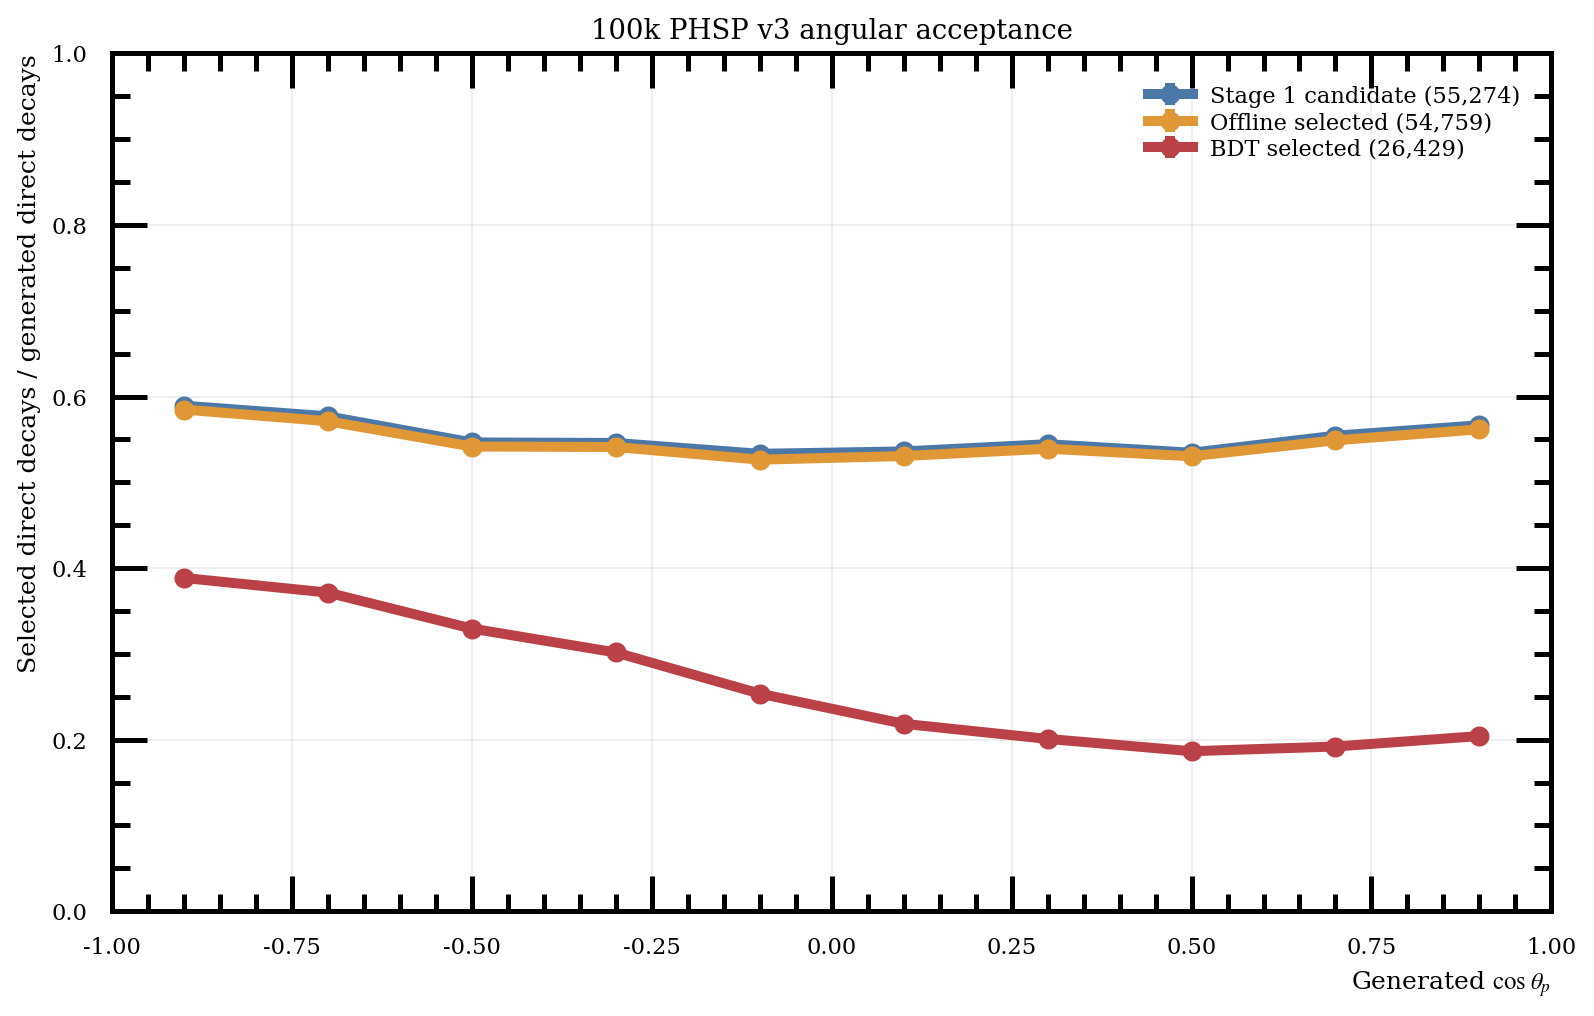
\includegraphics[height=.80\textheight]{figures/acceptance.png}
\end{frame}
\begin{frame}{Charge conjugates}
\centering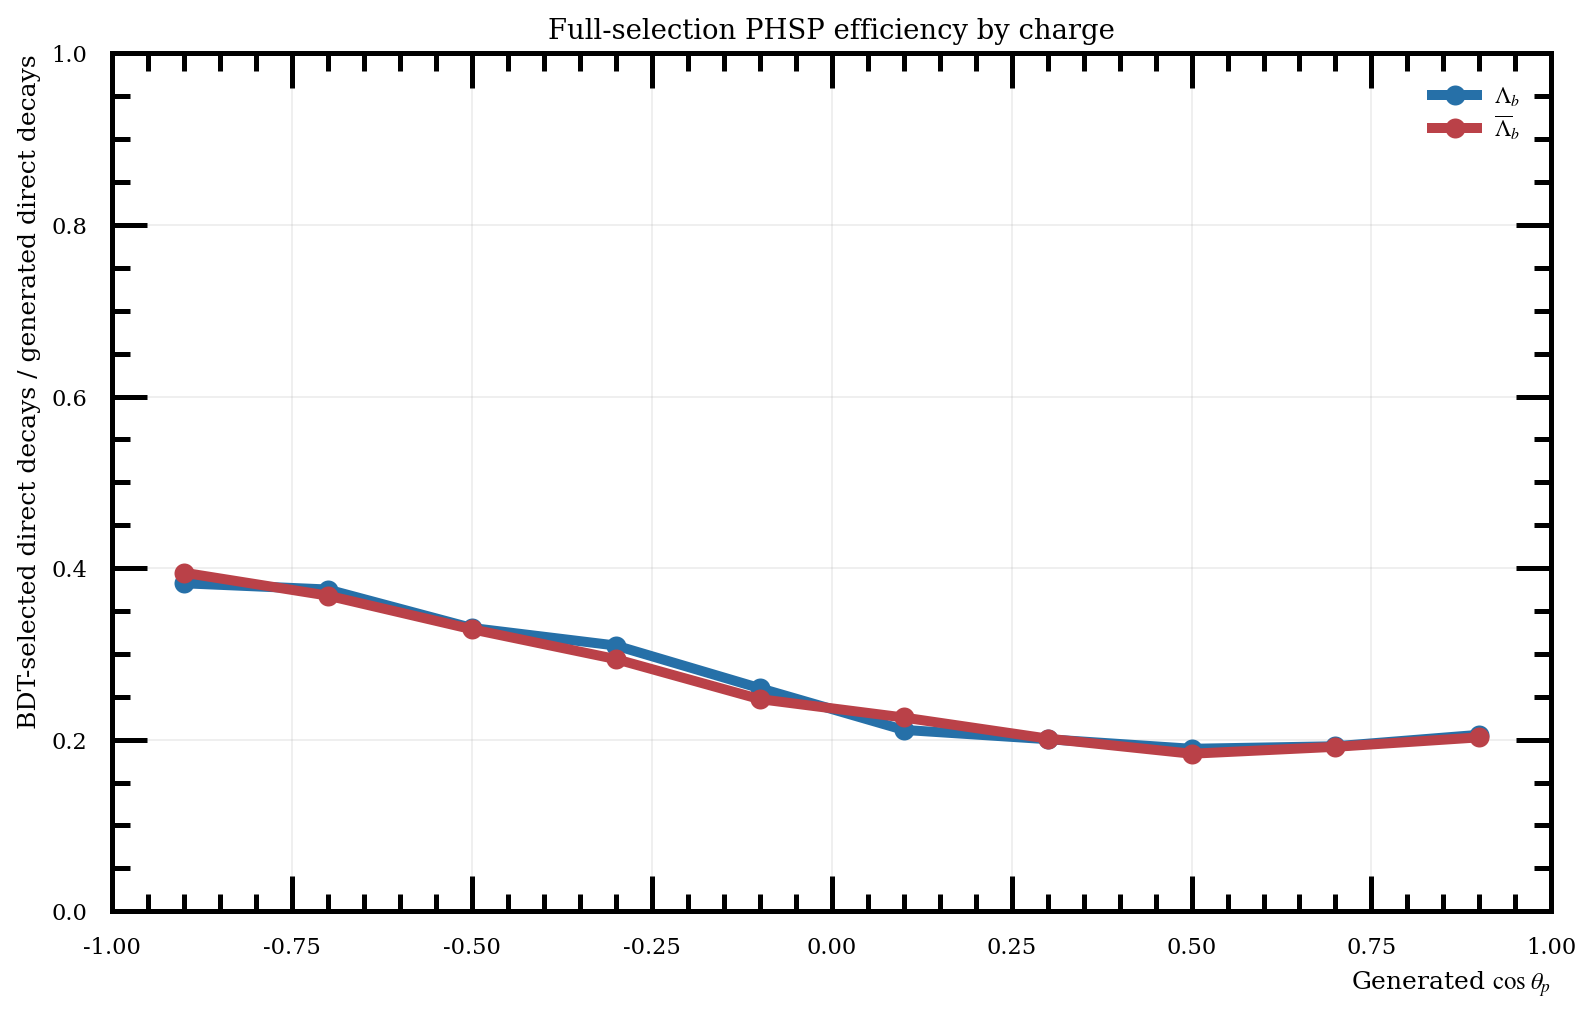
\includegraphics[height=.80\textheight]{figures/charge.png}
\end{frame}
\begin{frame}{Reconstructed minus generated angle}
\centering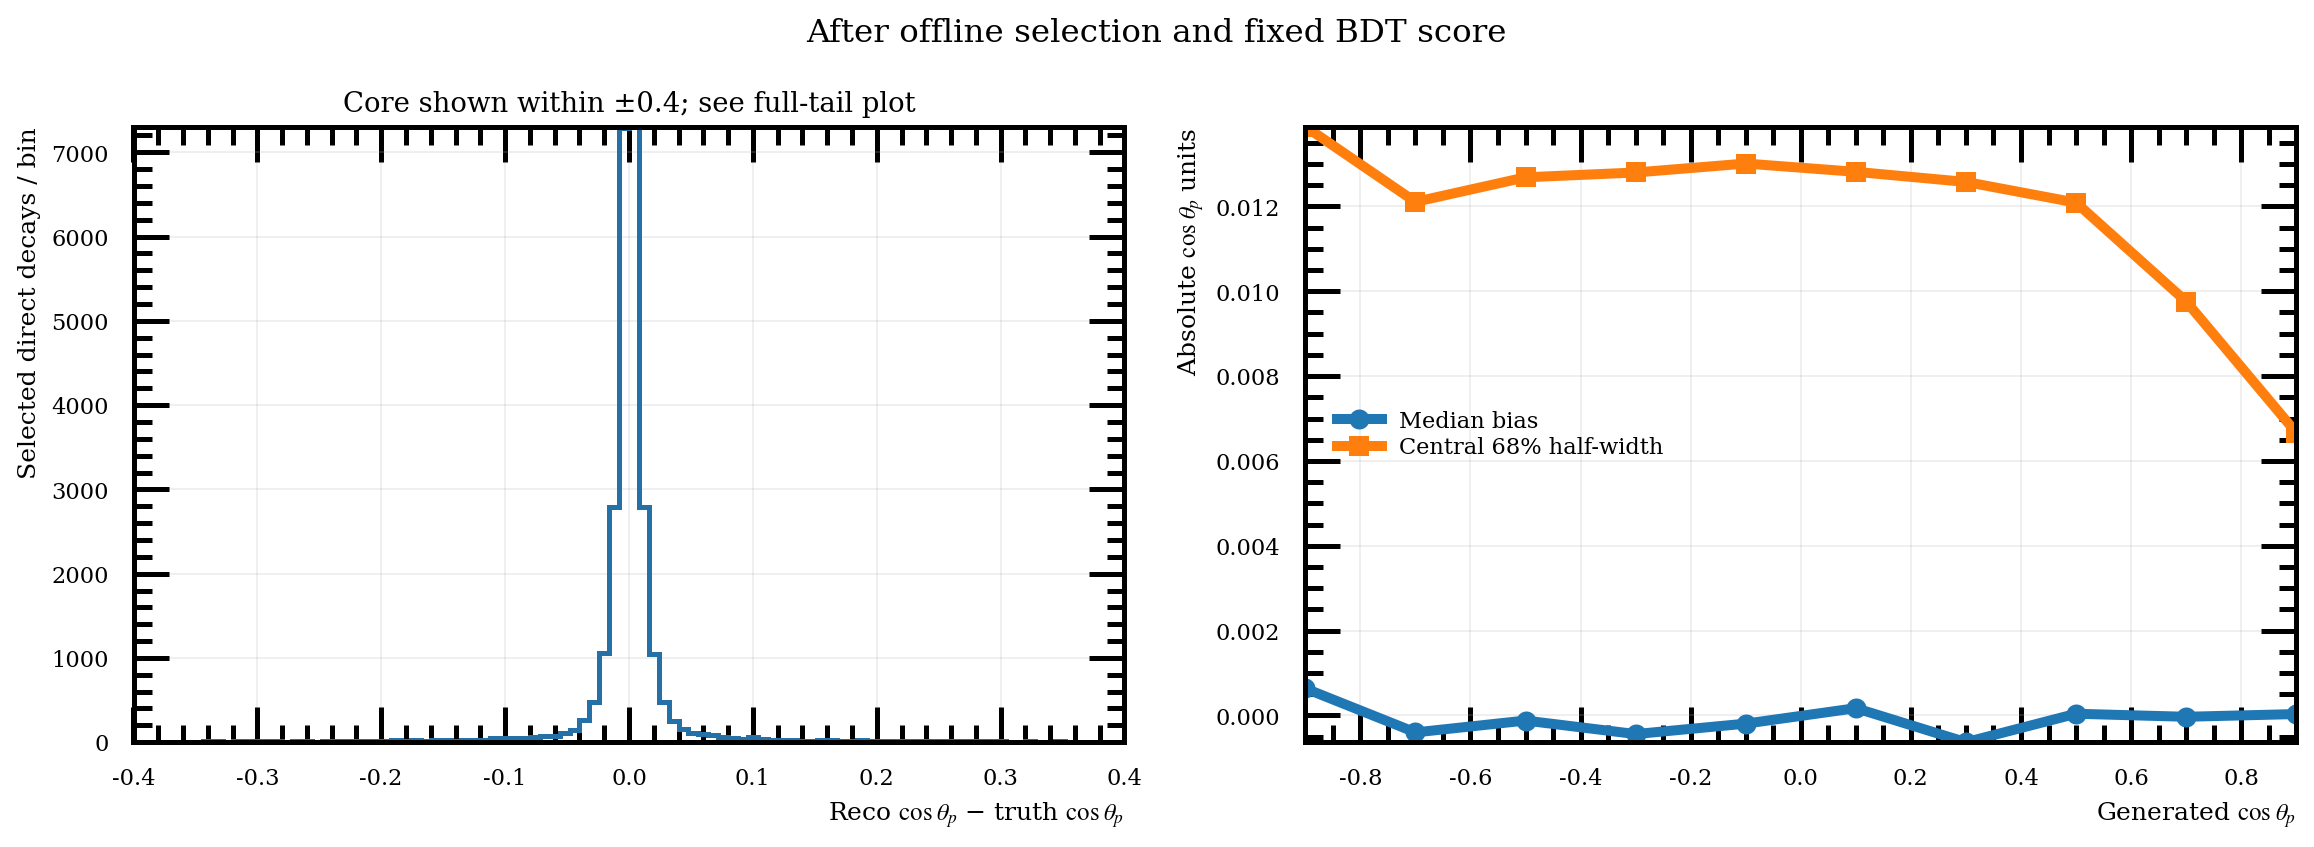
\includegraphics[height=.80\textheight]{figures/resolution.png}
\end{frame}
\begin{frame}{Migration for a binned angular fit}
\centering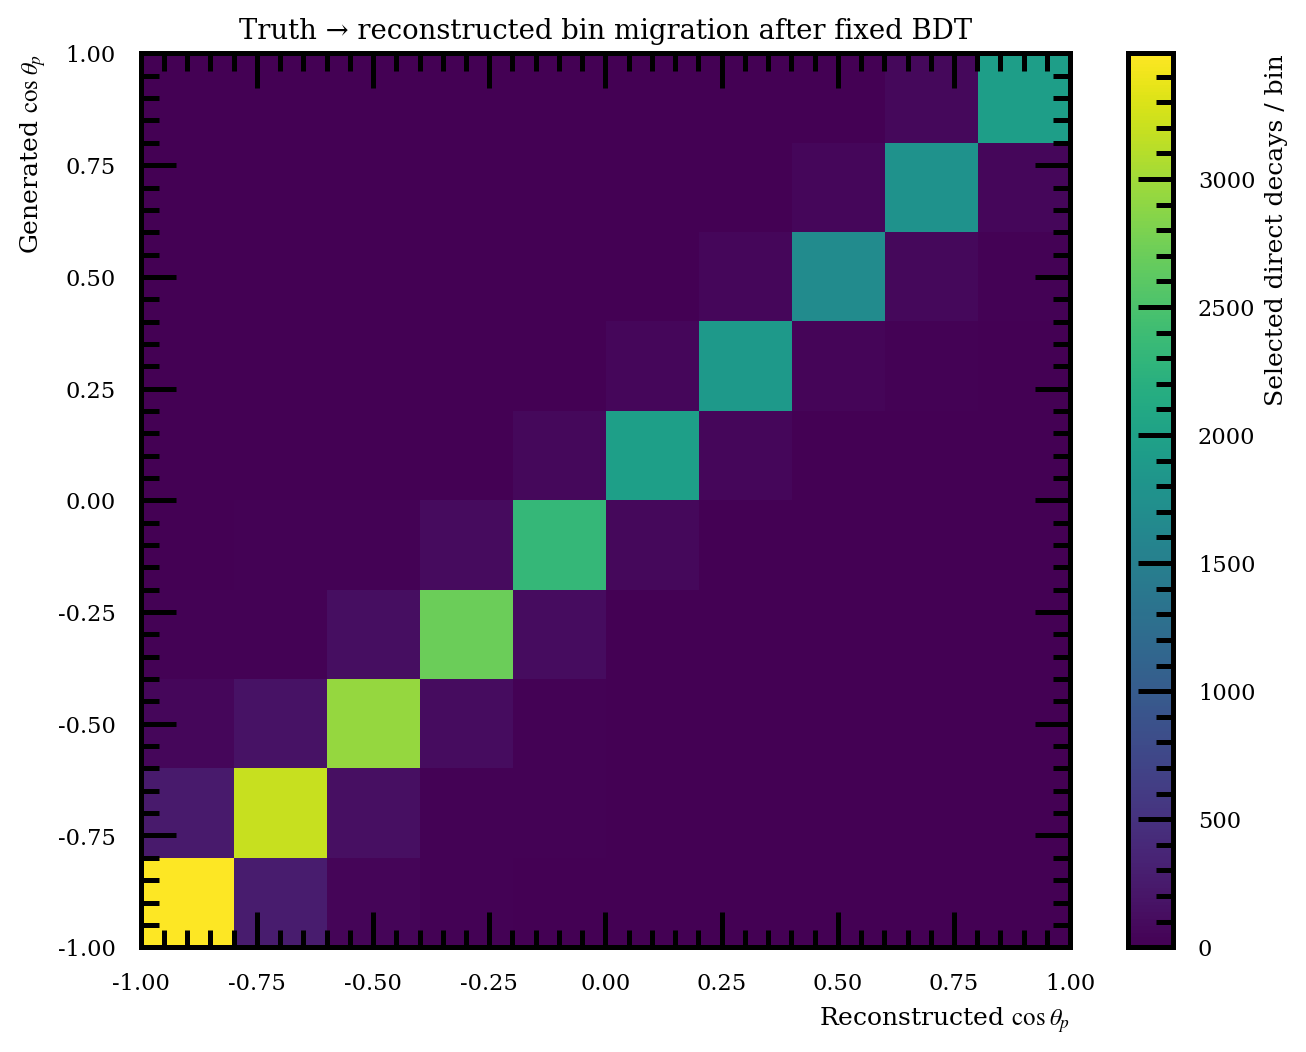
\includegraphics[height=.80\textheight]{figures/migration.png}
\end{frame}
\begin{frame}{Numerical summary and fit contract}
\small
\begin{tabular}{lrrr}
\toprule
Stage & Direct candidate rows & Unique direct decays & Cumulative efficiency\\
\midrule
Stage 1 & 55,294 & 55,274 & 55.27\%\\
Offline & 54,779 & 54,759 & 54.76\%\\
Fixed BDT & 26,436 & 26,429 & 26.43\%\\
\bottomrule
\end{tabular}
\vspace{.4em}
\begin{itemize}
\item BDT acceptance changes from 0.389 in the most negative truth bin to 0.186 in $0.4\leq\cos\theta_p<0.6$.
\item Selected residual: median $1.0\times10^{-5}$, central 68\% half-width 0.0118, RMS 0.0888; 5.6\% have $|\Delta\cos\theta_p|>0.1$.
\item Fit the generated angular shape after folding through the truth-row/reconstructed-column response matrix. Recompute if the score or model changes.
\end{itemize}
\end{frame}
\end{document}
